\documentclass[a4paper]{exam}
\usepackage[a4paper,
            bindingoffset=0.2in,
            left=1in,
            right=1in,
            top=1in,
            bottom=1in,
            footskip=.25in]{geometry}

\usepackage{amsfonts,amsmath,amsthm}
\usepackage{xcolor}
\usepackage{wasysym}

\usepackage{tikz}
\usepackage{tikz-qtree}


\newcommand\N{\ensuremath{\mathbb{N}}}
\newcommand\union{\cup}
\newcommand\interx{\cap}

\header{CS/MATH 113}{WC08: Induction}{Spring 2025}
\footer{}{Page \thepage\ of \numpages}{}
\runningheadrule
\runningfootrule

% \printanswers

\qformat{{\large\bf \thequestion. \thequestiontitle}\hfill}
\boxedpoints

\title{Weekly Challenge 08: Induction}
\author{CS/MATH 113 Discrete Mathematics}
\date{Spring 2025}

\begin{document}
\maketitle



\begin{questions}
    \titledquestion{Plagiarizing in Discrete Math} You surprisingly have more than two friends. Let $n$ be the number of friends you have. You and your friends have managed to get hold of solutions of Discrete Mathematics assignments through whatever means. Each of your friends have the solution of one such assignment. Now you need to share the solutions amongst yourselves, but your RAs are onto you and each of your communication is being monitored. But of course, there are only so many communications three RAs can monitor at a time, so it might very well be that some of the exchanges go undetected. Then again, you need to be safe. So to lower your chances of detection as much as possible, you need to minimize the number of exchanges. Also any gathering or communication between more than two students is always monitored, so only two students can communicate and share solutions with each other at a time. At any exchange, two of the students can share all the solutions they currently possess with each other. Prove or disprove the following claim: $2n-2$ exchanges are sufficient to share all the solutions to everyone in your friend group.



    \begin{figure}[!tbh]
        \centering
        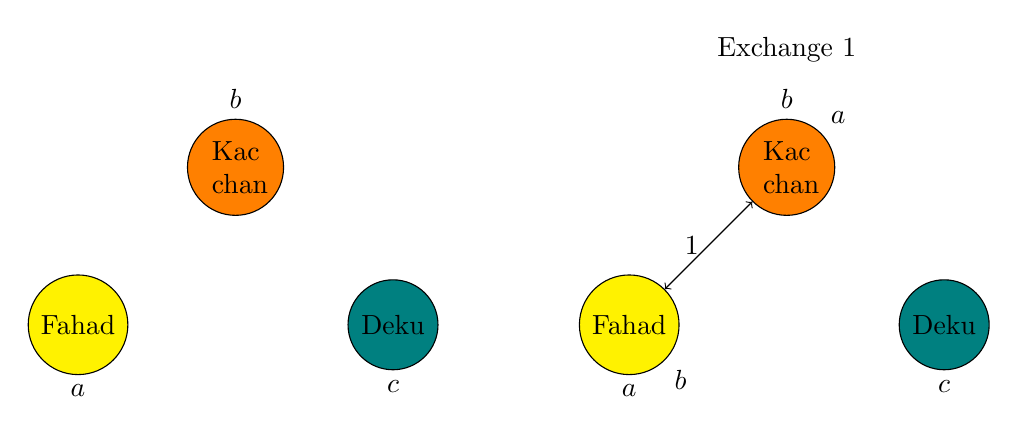
\begin{tikzpicture}
            \node [style={circle,draw, fill=yellow},label=below:$a$] (A) at (0,0) {Fahad};
            \node [style={circle,draw,text width=6mm, fill = orange},label=above:$b$] (B) at (2,2) {Kac\\chan};
            \node [style={circle,draw, fill = teal},label=below:$c$] (C) at (4,0) {Deku};

            
            \node [] (L) at (9,3.5) {Exchange 1};
            \node [style={circle,draw, fill = yellow},label=below:$a$,label=below right:$b$] (A1) at (7,0) {Fahad};
            \node [style={circle,draw,text width=6mm, fill = orange},label=above:$b$,label=above right:$a$] (B1) at (9,2) {Kac\\chan};
            \node [style={circle,draw},label=below:$c$, fill = teal] (C1) at (11,0) {Deku};
            \draw[<->] (A1) edge node[left] {1} (B1) ;


        \end{tikzpicture}
        
 \vspace{0.5cm}
 
        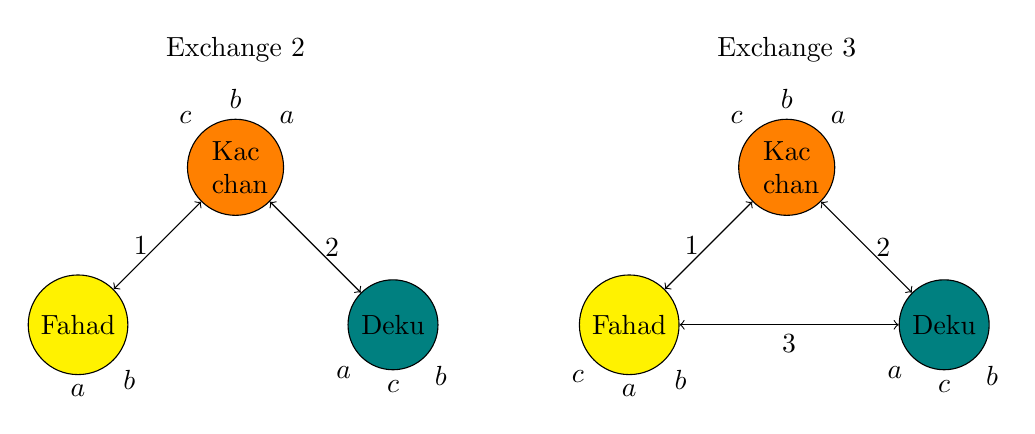
\begin{tikzpicture}
            \node [] (L) at (2,3.5) {Exchange 2};
            \node [style={circle,draw, fill = yellow},label=below:$a$,label=below right:$b$] (A) at (0,0) {Fahad};
            \node [style={circle,draw,text width=6mm, fill = orange},label=above:$b$,label=above right:$a$,label=above left:$c$] (B) at (2,2) {Kac\\chan};
            \node [style={circle,draw, fill = teal},label=below:$c$,label=below right:$b$, label=below left: $a$] (C) at (4,0) {Deku};
            \draw[<->] (A) edge node[left] {1} (B) ;
            \draw[<->] (B) edge node[right] {2} (C) ;

           
            
            \node [] (L) at (9,3.5) {Exchange 3};
            \node [style={circle,draw, fill = yellow},label=below:$a$,label=below right:$b$, label=below left:$c$] (A1) at (7,0) {Fahad};
            \node [style={circle,draw,text width=6mm, fill = orange},label=above:$b$,label=above right:$a$,label=above left:$c$] (B1) at (9,2) {Kac\\chan};
            \node [style={circle,draw, fill = teal},label=below:$c$,label=below right:$b$, label=below left: $a$] (C1) at (11,0) {Deku};
            \draw[<->] (A1) edge node[left] {1} (B1) ;
            \draw[<->] (B1) edge node[right] {2} (C1) ;
            \draw[<->] (C1) edge node[below] {3} (A1) ;

        \end{tikzpicture}
        
        \caption{An example of exchanges of solutions amongst three students, where Fahad start with solution $a$, Kacchan has solution $b$ and Deku has solution $c$.}
    \end{figure}

    \begin{solution}
        % Enter solution here.
    \end{solution}
    
\end{questions}

\end{document}
%%% Local Variables:
%%% mode: latex
%%% TeX-master: t
%%% End:


